Each command belongs to a service. 
Within that service, the command is identified by the \textit{sub-type} (a positive integer). 
Thus, a command is fully identified by a pair [x,y] where 'x' is the identifier of the service to which the command belongs (the service type, see section \ref{sec:ServConcept}) and 'y' is the identifier of the command within the service (the command sub-type).

Commands are \textit{types} which are instantiated at run-time. 
A command is generated by a service user in order to trigger the execution of certain actions by the service providers. Thus, a command instance begins its life when the application on the service user side (the \textit{user application}) decides that it wishes to issue a request to the application on the service provider side (the \textit{provider application}). 

A command is sent by the user application to the provider application where it triggers the execution of certain actions. Before being sent to the provider application, the command is configured. Through the configuration process, the command acquires the information it will need to execute its actions. The command's actions in the provider application are executed in a sequence of steps which may extend over time. Both the sending of the command to its destination and the execution of its actions in the provider application are conditional upon certain checks being passed. The command encapsulates both the actions that must be executed and the conditional checks that determine whether the command is sent and whether its actions are executed.

The same command instance may be sent to its destination more than once. This models the situation where a user is issuing periodic requests to a service provider. In this case, the content of the command is updated every time the command is sent to its destination. It is a logical error to re-send a command instance to its destination before the actions triggered by the previous execution of the same command have completed.

A command is defined by its \textit{attributes}, its \textit{conditional checks}, and its \textit{actions}. 

Attributes designate characteristics that are entirely defined by their value. 
Actions and conditional checks designate executable functionalities that are associated to the command. 
Both actions and conditional checks are executed by the command as a result of changes in its internal state. 
The conditional checks are used to determine whether and when the command actions are executed.

The next three subsections further define the command attributes, the command conditional checks, and the command actions. The last sub-section describes the lifecycle of a command. 

%---------------------------------------------------------------------------------
\subsubsection{The Command Attributes}\label{sec:CmdAttributes}

An attribute is a characteristics that is entirely defined by its value. 
A command has the following attributes:

\begin{itemize}
\item \textbf{Service Type:} Each command contributes to implementing a service. This attribute identifies the service that the command implements. 

\item \textbf{Command Sub-Type}: Each service is implemented by several commands. 
This attribute identifies the type of the command within a certain service. 

\item \textbf{Command Identifier}: A command may exist in two distinct applications (the user application which sends the command and the provider application which receives it). This attribute uniquely identifies the command instance within both applications and throughout the life of both applications.

\item \textbf{Destination} Commands are generated by a user application for a provider application. This attribute identifies the provider application for which the command is intended.

\item \textbf{Source}
Commands are generated by a user application for a provider application. This attribute identifies the user application which issues the command.

\item \textbf{Time Stamp}:
The time when the user application makes the request to send the command to its destination. 

\item \textbf{Group}
Commands sent by a user application to the same destination are allocated to a group. This attribute identifies the group to which the command belongs. The concept of group is primarily relevant to applications which aim at PUS-compliance (see section \ref{sec:RelationshipToPUS}). 

\item \textbf{Sequence Counter}
Every time a user application issues a command belonging to a certain destination group, it increments a counter. The sequence counter attribute holds the value of this counter. The sequence counter can be used by the recipient application to check whether any commands addressed to it have been lost. 

\item \textbf{Acknowledge Level}
Command execution goes through four stages: acceptance, start, progress, and termination (see section 5.1.4). This attribute determines whether successful completion of each of these stages should be reported to the sender of the command. Note that failure to complete a stage is reported unconditionally.

\item \textbf{Progress Step Identifier}
On the service provider side, a command is executed in a sequence of progress steps. Each progress step is identified by a positive integer (but note that step identifiers are not necessarily in sequence). This attribute holds the identifier of the current step. A command must have at least one step. This attribute is only meaningful on the service provider side.

\item \textbf{Command Parameters}
Some commands may require parameters to fully specify the actions and checks that they encapsulate. The “Command Parameters” attribute holds the value of these parameters. This attribute consists of an ordered sequence of items of primitive type. 

\item \textbf{Discriminant}
The number and type of command parameters in a command instance is not necessarily determined by the command type (i.e. different instances of the same command type may have different sets of command parameters). The discriminant is a command parameter which determines the number and type of the other command parameters. 

Thus, the layout of a command instance is fully determined by the triplet: [x,y,z] where 'x' is the identifier of the service to which the command belongs (the service type), 'y' is the identifier of the command within the service (the command sub-type), and 'z' is the discriminant. 

The discriminant is an optional attribute. Command types which have no parameters, or which have a fixed set of parameters, have no discriminant.

\item \textbf{CRC}
A command carries a checksum which is set by the command's sender and which the recipient of the command can use to verify the integrity of the command's transmission. 
\end{itemize}

%---------------------------------------------------------------------------------
\subsubsection{The Command Conditional Checks}\label{sec:CmdCondChecks}

A conditional check is an executable functionality which returns an enumerated value. The enumerated value reports the outcome of the check. Conditional checks are performed as part of the processing of a command. Their outcome determines whether and when the command actions are preformed. Conditional checks must have zero logical execution time. This restriction allows them to be mapped to guards in state machines. 

Some checks are performed on the user's side (i.e. prior to the command being issued by the user application); others are performed on the provider's side (i.e. after the command has been received by the provider application). 

The following conditional checks are defined for a command on the service user side:

\begin{itemize}
\item \textbf{Enable Check}
This check is performed when the user application makes a request to send a command to the service provider. The enable check determines whether the command instance is enabled or disabled. If the command instance is disabled, then the command is aborted. If instead the command instance is enabled, it remains in a pending state until the ready check authorizes it being sent to its destination.

\item \textbf{Ready Check}
This check is performed on a pending command instance that has passed its enable check. The ready check determines when the command instance is sent to its destination.  The command instance remains pending until the ready check is passed. When the ready check is passed, the command instance may be sent to its destination. 

\item \textbf{Repeat Check}
This check is performed on a command instance after it has been sent to its destination. The check returns either "repeat" or "no repeat". In the former case, the command instance is updated and sent again to its destination. In the latter case, it is terminated.
\end{itemize}

On the service provider side, the following conditional checks are defined for a command:

\begin{itemize}
\item \textbf{Acceptance Check}
The acceptance check is performed when the command instance is received by its destination. If the acceptance check is passed, then the command remains pending and can be further processed by its recipient. If the acceptance check is not passed, then the command instance is aborted.

\item \textbf{Ready Check}
This check is performed on a pending command instance that has passed its acceptance check. The ready check determines when the execution of the command starts.  As long as the ready check is not passed, the command remains pending. When the ready check is passed, the command instance attempts to start execution.
\end{itemize}

%---------------------------------------------------------------------------------
\subsubsection{The Command Actions}\label{sec:CmdActions}
Command actions are executable functionalities which encapsulate the actions to be performed by the command. Command actions are executed depending on the outcome of the command conditional checks. Command actions must have zero logical execution time. This restriction allows them to be mapped to actions in state machines. 

The following action is defined for a command on the service user side:

\begin{itemize}
\item \textbf{Update Action}
Through this action, the command acquires the information which it requires to execute its action on the service provider application. This action is executed before the command is sent to its destination. If the command is sent more than once (i.e. if its repeat check returns "repeat" one or more times), then the Update Action is performed repeatedly every time the command must be sent to its destination.
\end{itemize} 

The following actions are defined for a command on the service provider side:

\begin{itemize}
\item \textbf{Start Action}
The start action is executed after the start check has been passed. The start action encapsulates one-off initialization actions that must be performed at the beginning of a command's execution. 
The start action has an outcome which is either “success” or “failed”. If the outcome of the start action is “failed”, the command is aborted. 
\item \textbf{Progress Action}
Commands execute in one or more execution steps. The progress action encapsulates the actions performed in one execution step. The progress action is executed the first time after the start action has terminated and it is then executed again until either it fails or it completes.
 
The progress action has two outcomes: a completion outcome which can be either "completed" or "not completed" and a success outcome which can be either "success" or "failed". If the completion outcome is "completed", then all execution steps have been completed and the termination action is executed. If, instead, it is "not completed", then another execution step will be executed. The success outcome determines the kind of acknowledge reports which are generated for the progress action. 

Finally, the progress action updates the progress step identifier. A "progress step" is a set of logically related execution steps which are executed in sequence.
\item \textbf{Termination Action}
The termination action is executed after all the progress steps have been successfully executed. The termination action encapsulates one-off finalization actions that must be performed before the command is terminated.
The termination action has an outcome which is either “success” or “failed”. If the outcome of the termination action is “failed”, the command is aborted. 
\item \textbf{Abort Action}
If a command is aborted (i.e. if it fails its acceptance check, or its start action faisl, or its progress action fails, or its termination action fails) then it executes its abort action. The abort action thus encapsulates the finalization actions to be performed in case of a command failure. 
\end{itemize}

%---------------------------------------------------------------------------------
\subsubsection{Command Lifecycle}\label{sec:CmdLifecycle}
A command instance begins its life on the user side when the user application makes a request for the command instance to be sent to the provider application. Nominally, on the user side, the command can be in one single state PENDING. This corresponds to the state of a command that has passed its enable check and is waiting for its ready check to authorize the transfer of the command to the provider application. 

On the provider side, the command instance passes through four states: ACCEPTED, STARTED, PROGRESS, and TERMINATED. The command states are entered in sequence as the command is executed. The PROGRESS state can be entered more than once to represent the fact that some commands execute actions which extend over time and which are therefore broken into several steps.

To each command state one check and one action may be associated. The checks determine whether a state can be entered or exited. For instance, if the acceptance check fails, then the command cannot be executed. The actions encapsulate the activities to be performed when the command enters a certain state. For instance, the start action defines the actions to be executed when the command is started. Actions have an outcome which determines the next step in the execution of the command.

On the provider side, a change in the state of a command is marked by the generation of an Acknowledge Report. Acknowledge Reports are used to notify the sender of a command of a change in the state of the command. Four kinds of Acknowledge Reports are defined corresponding to the four states that a command may have in a provider application:

\begin{itemize}
\item \textit{Acceptance Acknowledge Report} to notify the command sender of the outcome of the acceptance check.
\item \textit{Start Acknowledge Report} to notify the command sender of the outcome of the start action.
\item \textit{Progress Acknowledge Report} to notify the command sender of the outcome of a progress step.
\item \textit{Termination Acknowledge Report} to notify the command sender of the outcome of the termination action.
\end{itemize}

The sending of an acknowledge report to a command sender is done unconditionally in the following cases: (a) the acceptance check has not been passed, (b) the start action has failed, (c) the progress action has failed, or (d) the termination action has failed. Note that all of these cases result in the command being aborted. Thus, the sending of an acknowledge report is done unconditionally whenever a check or action results in a command being aborted. For instance, if the start action of a command fails, a Start Acknowledge Report is sent to the command sender to notify it that the command has failed to start execution and has consequently been aborted.

In all other cases (namely when the acceptance check is passed, or the start action, or the progress action, or the termination action are successful), the sending of the acknowledge report to the command sender is conditional upon the value of the Acknowledge Level attribute of the command (see section \ref{sec:CmdAttributes}). Thus, for instance, the command sender can set the Acknowledge Level attribute of a certain command such that only successful acceptance and successful termination of the command are reported. 

The Progress Acknowledge Report is only sent at the end of a progress step. A progress step is deemed to have ended when the previous execution of the progress action has resulted in the progress step identifier being updated.

Figure \ref{fig:CmdLifecycle} shows the nominal lifecycle of a command in an informal notation. In summary, the CORDET Framework pre-defines the logic to handle the transitions between the command states. It does this by defining the logic to manage the execution of the command checks and of the command actions but it leaves the definition of the content of the actions and checks open. 

The lifecycle outlined above may be repeated more than once for the same command instance. Repetition is determed by the outcome of the Repeat Check. The Repeat Check is performed at the end of the lifecycle depicted in figure \ref{fig:CmdLifecycle}. If it returns "no repeat", then the command instance is destroyed. If instead, the check returns "repeat", then the content of the command is updated and thze command is re-sent to its destination where it repeats the lifecycle of figure \ref{fig:CmdLifecycle}.

\begin{figure}[ht]
 \centering
 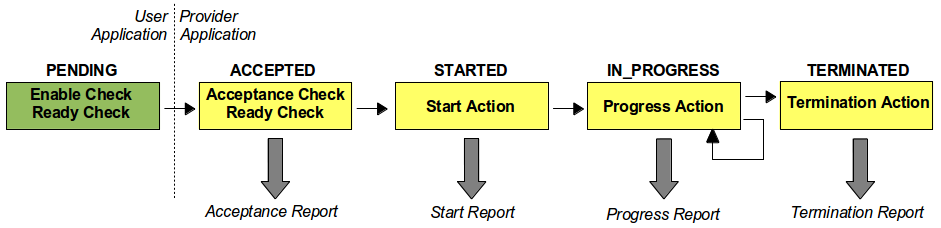
\includegraphics[scale=0.4,keepaspectratio=true]{CmdLifecycle.png}
 \caption{Command Lifecycle (Informal Notation)}
 \label{fig:CmdLifecycle}
\end{figure}


